\section{Modeling of Duplicate Bug Reports Detection}
%\section{Problem Formulation}
\label{formulation}

%Since the model is adapted from RTM~\cite{???}, in the text, we use
%some notations originated in~\cite{???}

We propose to use a topic modeling approach for the automatic
detection of duplicate bug reports. We utilize and adapt a
probabilistic, generative topic model called {\em Relational Topic
  Model (RTM)}~\cite{RTM} for the analysis and inference of the hidden
technical topics within bug reports and the relation of duplicate
reports based on their topics.

%\vspace{0.04in}
%\noindent\textbf{Overview.} This section describes our formulation for
%the problem of detecting duplicate bug reports. In our approach,
Each system is considered to have a number of (technical)
aspects. The bug database is considered as a collection of bug
reports. Each aspect of the system is considered as a topic of that
collection, represented via a set of certain words/terms. Each bug
report is considered as a textual document containing a number of
words/terms to report on some of those technical aspects. Among them,
some aspects might be incorrectly implemented with respect to the
system's requirements, thus, causing the bugs being reported. Two bug
reports are considered to be duplicate if they similarly describe the
same buggy topic(s). From now on, we use the terms (technical)
``aspect'' and ``topic'' interchangeably. The same treatment is for
``bug report'' and ``document'', and ``word'' and ``term''.

Since a document is a bug report, their topics with higher proportions
are more likely to be buggy or highly relevant to the buggy
topics. Other topics might have zero or very low proportion. If two
documents are duplicate, i.e. reporting the same buggy topics, their
corresponding topic proportions of those common topics would be high
in both reports. If two documents are not duplicate bug reports, the
two topic proportions might not be much similar (i.e. the distribution
values of common topics might not be high in both documents).

%
%To formulate the duplicate bug reports detection problem, we develop a
%parameterized, probabilistic, generative model. We call it
%\emph{incremental Relational Topic Model (iRTM)} because we extend the
%original RTM~\cite{RTM} for this detection problem. The key ideas of
%{\model} include:

%1) it considers bug reports as the observations which arise from a
%generative, probabilistic process with hidden variables. For this
%problem, the collection of bug reports including duplicate ones is
%modeled as to be {\em generated} by {\model} model;

%2) via training on historical data, for example the already-identified
%   as duplicate bug reports, it {\em estimates} those hidden variables
%   using posterior inference;

%3) then it situates new data into the estimated model, i.e., it will
%   predict {\em how likely a new bug report and an existing one are
%   generated by the estimated model} to determine whether they are
%   duplicate ones; and

%4) The trained model is quickly updated via our incremental algorithms
%   (Section~IV) without fully re-training as new bug reports arrive.

\begin{figure}[t]
\centering
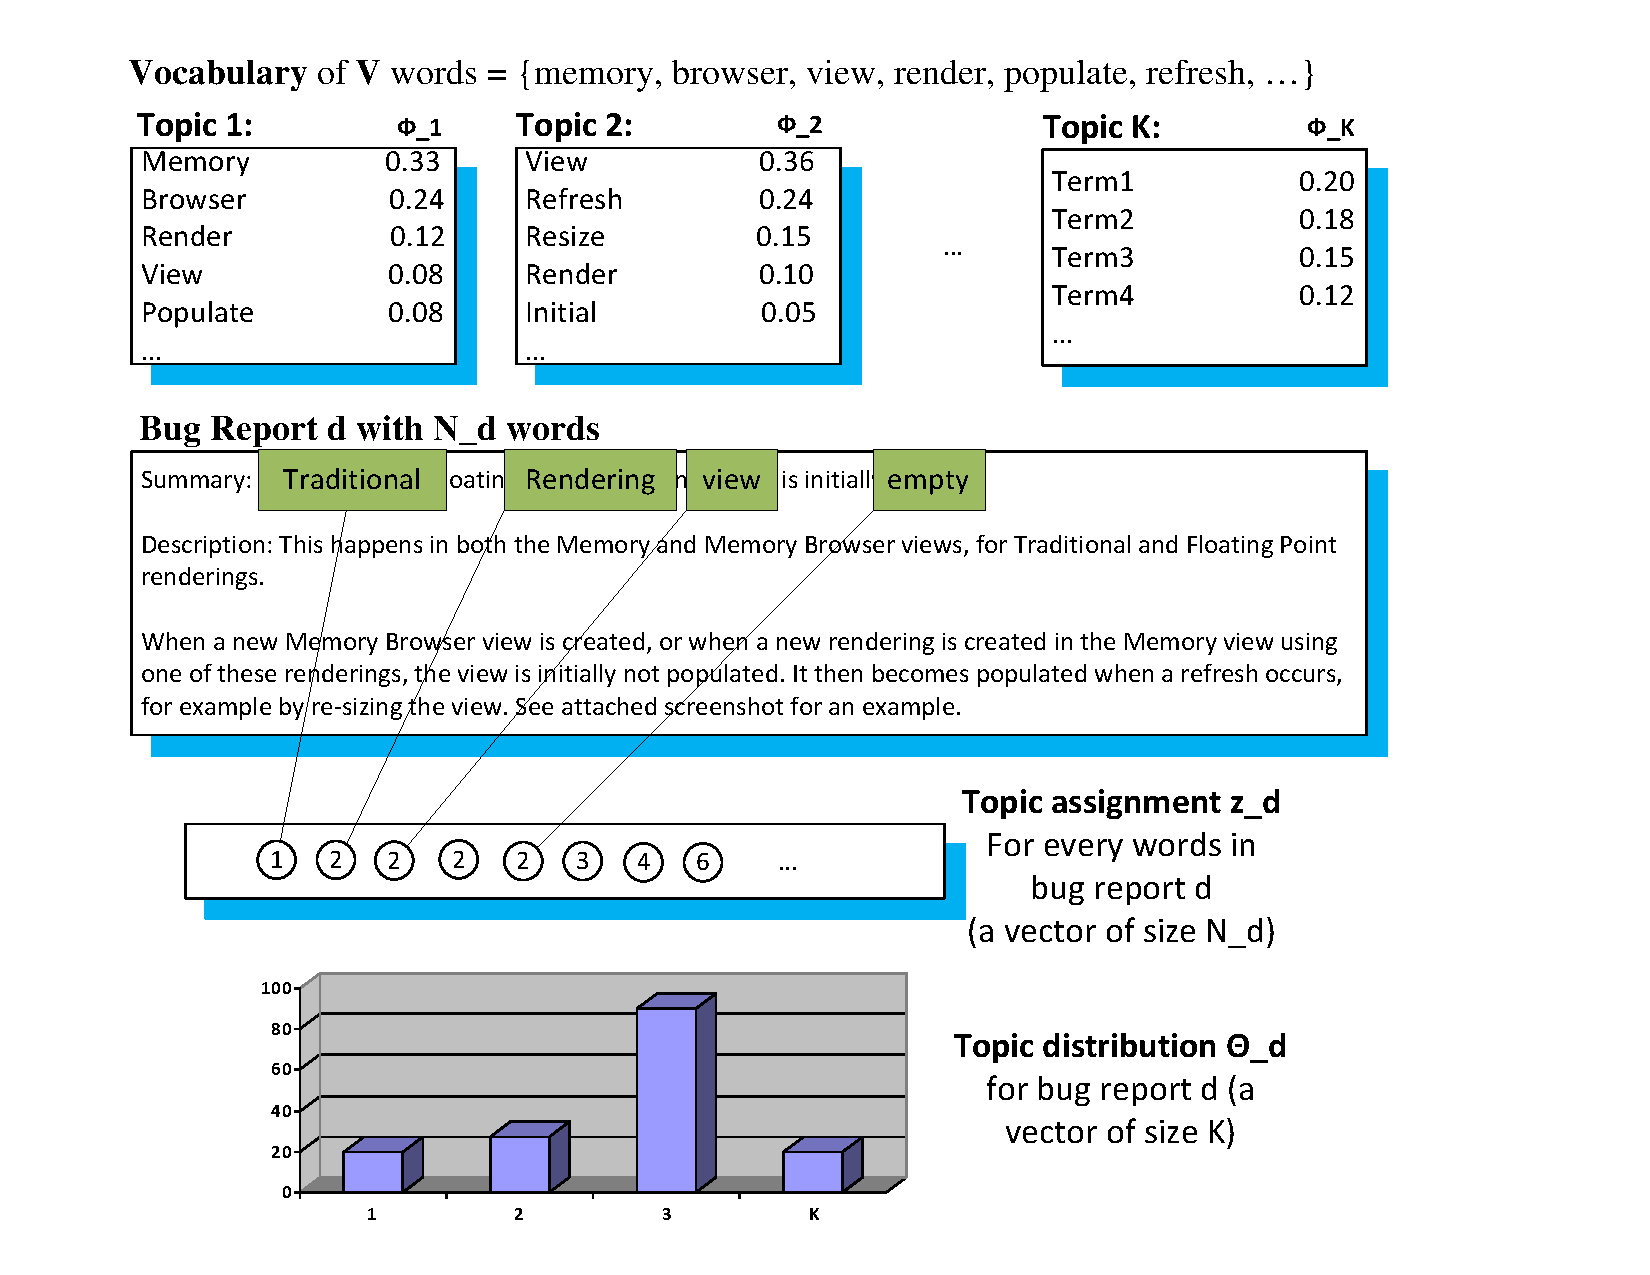
\includegraphics[width=4.2in]{irtm4}
\caption{Topic Modeling for Bug Reports~\cite{lda}}
\label{topicmodel}
\end{figure}

%\subsection{Relational Topic Modeling}


%For topic modeling in bug reports, we use LDA~\cite{lda} and adapt
%RTM~\cite{RTM}. 

%We formulate the problem of duplicate bug report detection by
%adapting RTM~\cite{RTM}.

Figure~\ref{topicmodel} shows the details.  The global
parameters include a vocabulary containing $V$ words available to be
used in the bug reports and a set of $K$ topics. The topic indexed by
$t$ ($t=1..K$) is modeled by a vector $\phi_t$ of size $V$, in which
$\phi_{t,x}$ is the probability that word $x$ in the vocabulary is
used to describe topic $t$.

A document $d$ generated by this model is considered as a sequence of
$N_d$ words, describing a mixture of such topics. The mixture, called
{\em topic distribution}, is represented by a vector $\theta_d$ of
size $K$. $\theta_{d,t}$ is the proportion of topic $t$, i.e. there
are expectedly $\theta_{d,t}*N_d$ words in document $d$ describing
topic $t$. Each position within $d$ is used to describe one topic. The
topic assignment for such positions is represented by a vector $z_d$
of size $N_d$, in which $z_{d,n}$, having value in 1..$K$, is the
index of the topic that the word $n^{th}$ in document $d$ describes.

%-------------------------------------------------------------------
\vspace{0.04in}
\noindent {\bf Duplication Indicator.} 
RTM is adapted to model the duplication relation among bug
reports. For two bug reports $d$ and $d'$, a {\em duplication
indicator} $y_{d,d'}$, will be set to 1 if they are duplicate, and 0
otherwise. Because we determine the duplication of two bug reports
based on how similarly they describe the same buggy topics, we define
a function $\psi(d,d')$ to measure the topic-based similarity of two
documents and determine the value of $y_{d,d'}$ based on
$\psi(d,d')$. That is, the higher $\psi(d,d')$ is, the higher
probability that $d$ and $d'$ are duplicate bug reports. In this
context, $\psi$ is called the {\em duplication indicating
function}. As suggested in~\cite{RTM}, we use the following function:
$$\psi(d, d') = exp({\sum\nolimits_{k=1}^K(\eta_k.\theta_{d,k}.\theta_{d',k})+
\nu})$$ in which $\eta_k$s are the weighted parameters and $\nu$ is a
smoothening parameter. As seen, this function measures the similarity of
the two documents via their topics. First, it calculates the
similarity of their topics via a weighted product of the corresponding
topic distribution vectors $\theta_d$ and $\theta_{d'}$. Then, it uses
an exponential function to amplify such similarity of those
vectors to calculate the desired topic-based similarity ($\psi(d,d')$)
between those two documents.

If two documents report the same buggy topics, their corresponding
topic distribution values of those common topics would be high in both
vectors, leading to the high weighted product and high duplication
indicating value returned in the formula via the exponential function.
If two documents are not duplicate bug reports, i.e. the distribution
values of common topics might not be high in both vectors, thus, the
weighted product and the duplication indicating value would be low.

%The correlation between this function and the duplication indicator
%could be understood intuitively as follows. Since a document is a
%bug report, their topics with higher proportions are more likely to be
%buggy or highly relevant to the buggy topics. Other topics might have
%zero or very low distribution. If two documents are duplicate,
%i.e. reporting the same buggy topics, their topic distributions might
%not be the same. However, their corresponding topic distribution
%values of those common topics would be high in both vectors, leading
%to the high weighted product and high duplication indicating value
%returned in the formula via the exponential function. Otherwise, if
%two documents are not duplicate bug reports, the two vectors might not
%be much similar (i.e. the distribution values of common topics might
%not be high in both vectors), thus, the weighted product and the
%duplication indicating value would be low.

%\vspace{0.03in}\noindent\textbf{Generation Process.}
%Formally, based on its parameters, RTM considers that the bug reports
%and their duplication indicators are generated according to the
%following probabilistic process:

%1. Choose the vocabulary of size $V$, the number of topics $K$, the
%   number of documents $M$, and the other per-collection parameters
%   $\alpha$, $\beta$, $\eta$, and $\nu$.

%2. Choose the per-topic term distributions. For each topic $t$ in
%1..$K$, draw $\phi_t$ following Dirichlet distribution
%$Dir(\beta,V)$, i.e., $\phi_t \sim Dir(\beta,V)$. Each sample of
%$Dir(\beta,V)$ is a vector of $V$ non-negative elements that are
%summed up to 1.

%3. For each document $d$ in the range of 1..$M$:

%3.1. Choose the per-document topic distribution $\theta_d$ of document
%     $d$: $\theta_d \sim Dir(\alpha, K)$. $\theta_d$ is a vector $K$
%     non-negative elements, summed up to 1, and $\theta_{d,t}$ is the
%     relative proportion of the words that are used for topic $t$ in
%     document $d$.

%3.2. Choose the size of document $N_d$ following Poisson
%     distribution as in ~\cite{RTM}.

%3.3. Choose the per-document topic assignment $z_d$ of document
%     $d$. $z_d$ is a vector of $N_d$ integer elements. The $n^{th}$
%     element is the index of the topic assigned for the $n^{th}$ word
%     in $d$. Since $d$ has topic distribution $\theta_d$,
%     $z_{d,n} \sim Multinomial(\theta_d)$.

%3.4. Generate the words $w_d$ of document $d$. $w_d$ is a vector of $N_d$
%     elements, in which $w_{d,n}$ is the index in the vocabulary of
%     the concrete word at the $n^{th}$ position of $d$. Since the
%     word at the $n^{th}$ position is assigned to topic $z_{d,n}$,
%     $w_{d,n}$ is drawn based on the per-topic term distribution
%     $\phi_{z_{d,n}}$: $w_{d,n} \sim Multinomial(\phi_{z_{d,n}})$.

%3.5. Generate the duplication indicators of document $d$ with respect
%     to other generated documents. For each generated document $d'$
%     with topic proportion $\theta_{d'}$, if $\psi(d, d')$ is sufficiently large
%     then $y_{d,d'} = 1$, otherwise $y_{d,d'} = 0$.

%Note that this is a hypothesized process from the point of view of a
%machine learning mechanism for the generation of bug reports including
%the duplicated ones. This process is used for the training and
%prediction purpose in {\model}. It does not imply a real-life process
%of bug reporting.


%\subsection{{\model} for Incremental Training and Inferring}

%Let us describe our extension to RTM for the bug report duplication
%detection. In {\model}, we use the above process to model the
%generation of the collection of bug reports including the duplicate
%ones. Therefore, we could detect duplicate bug reports by following
%step 3.5. However, we can observe only the words in bug reports,
%i.e. vector $w_d$, and some manually detected duplication indicators
%$y_{d,d'}$ for some pairs of bug reports that have been recorded in
%the history. Thus, to detect the unobserved duplication indicators of
%other pairs, we need to infer the hidden parameters of the collection
%including 1) the per-topic term distribution $\phi_t$ for the whole
%collection, 2) the per-document topic distribution $\theta_d$, and 3)
%the per-word topic assignment $z_d$ of each document. This inferring
%process must also take into account new information on reports and
%their duplications to update its inferred parameters. The reason is
%that in software evolution, new bug reports are filed continually and
%duplicate reports are also newly identified (for both old and new
%reports). Thus, there are three phases in {\model}:


%\item {\bf Initial training}.  Documents ($w_d$s) and recorded
%duplication indicators ($y_{d,d'}$s) are provided. {\model} is
%trained to get topic structures ($\phi_t$ for each $t$) of the
%collection, and that of each document ($\theta_d$ and $z_d$ for
%each~$d$).

%\vspace{0.05in}
%\item {\bf Detecting}.  In this phase, a document $d$ is provided. This
%document might be an already-filed or a newly filed bug report. We
%detect whether it is a duplicate report of another filed report. Thus,
%the model is used to infer the topic structures of the report
%($\theta_d$ and $z_d$, if needed, e.g. for a new report), and more
%importantly, its duplication indicators ($y_{d,d'}$) to all other
%documents. The inferred indicators, i.e. potential duplications, are
%reported to the users for manual verification.

%\item {\bf Updating}.  In practice, the bug reports are constantly
%  filed. New information on the duplicate reports is also provided.
%  This information includes new bug reports and duplication indicators
%  (including the indicators verified after the detecting phase, or new
%  indicators that are manually identified by users). For example, the
%  users could manually identify some new duplicate bug reports. They
% could verify some of the automatically detected duplications by our
%  tool as true duplications. The model, thus, needs to be updated with
%  newly available information. Otherwise, if the initially trained
%  model is used to process new data, that model might not fit well.

%A naive updating method is to completely re-train the model on both
%already-trained and newly available data. Since the new data is
%provided with high rate and volume, and the trained data is also of
%high volume, this naive approach would be very inefficient. On the
%other hand, if we train the model with only new data, we might miss
%the potential duplications between the new and the existing bug
%reports. Thus, our balanced approach is to select a representative
%portion of existing data to re-train with new data and use the trained
%information to update the global parameters (e.g. per-topic word
%distribution) as suggested in~\cite{canini09}. We will explain how our
%model {\model} will update its recently trained parameters such as
%$\phi_t$, $\theta_d$, $z_d$ in the next section.

%\end{enumerate}


